\chapter{Clustering Analysis (CA)}
\label{appendix_a}
\bibliographystyle{nar}
\section{General Methodology}
We considered  each of  the 20 non-A-RNA  type structures as  a vector
composed of  six base-step  parameters.  We group these  vectors using
cluster analysis  following an automated process  shown to succesfully
reproduce well  known patterns of  the Periodic Table from  a selected
set  of variables, such  as, electronegativity,  ionization potential,
and  other elemental  properties  \cite{restrepo2004}.  The  procedure
followed  here  is  an  adaptation   of  how  clustering  is  used  to
re-construct the Periodic Table classification of the elements.

We start by normalizing the vectors of step parameters,
\begin{gather}
\label{eq:normalization}  
\overline{x}_{jA}=\frac{x_{jA}-x_{jmin}}{x_{jmax}-x_{jmin}}
\end{gather}
where ${x}_{jA}$ is the value  of the step parameter \textit{j} of the
structure A and $x_{jmin}$ and  $x_{jmax}$ are the minimum and maximum
values for a particular step parameter \textit{j} \cite{restrepo2006}.
Then,  using  the  software  package \textsf{R}  \cite{ihaka1996},  we
cluster these vectors into groups.  These groups can be displayed in a
tree  representation,  also called  a  dendrogram,  or  in biology,  a
phylogenetic tree (see Figure~\ref{fig:tree}).

To cluster these vectors into groups, it is necessary to define the
distance between  the vectors. In  this work we used  three distance
definitions.   These distances  are  often referred  to as  Manhattan,
Euclidean  and   maximum  distances.  The  first   two  distances  are
particular cases of what is known as Minkowski's metric:
\begin{gather}
d(X,Y)= \Big( \sum_{i=1}^N |x_i-y_i|^k \Big)^\frac{1}{k}
\end{gather}
where $d(X,Y)$ refers to the distance between two vectors $X$ and $Y$,
where $N$ is  the dimensionality of the vector.  For  the case of step
parameters, $N$ is  six.  In the case where \textit{k}  is equal to 1,
the  definition  corresponds to  the  Manhattan  distance (a  distance
measured by  following along the edges  of blocks). In  the case where
\textit{k} is equal to 2, we have the familiar Euclidean distance. The
remaining distance, that is, the maximum distance, is defined by:
\begin{gather}
d(X,Y) = max |x_{i}-y_{i}|
\end{gather}
where  the  distance  between  vectors  $X$ and  $Y$  is  the  maximum
difference between vector variables.

Yet  another distance  definition used  in  this text,  which is  more
frequently interpreted as an statistical measure of error, is the root
mean square  deviation (RMSD). The  root mean square deviation  can be
seen as a  mean euclidean distance, in the sense  that it's defined as
the square  root of the ratio  between the sum  of squared differences
between vector variables, and the dimensionality of the vectors $N$.

\begin{gather}
RMSD(X,Y)      =     \Big(      \frac{\sum_{i=1}^2     |x_i-y_i|^2}{N}
\Big)^\frac{1}{2} \label{eq:rmsd}
\end{gather}

%\noindent
Once the  distance is defined, we use  a hierarchical method
to cluster  the set of distances between  base-step parameters.  The
clustering algorithm first finds the two closest vectors (given by one
of  the  distance definitions)  and  groups  them  together.  Then  it
compares the  distance of the elements  in the newly  formed group and
the  elements remaining  to be  grouped, according  to  the particular
clustering method.  For example,  the single linkage clustering method
takes  the  minimum  distance   between  elements  as  the  clustering
criterion.  Such an approach would, as all other agglomerative
hierarchical methods do, group together the closest vectors given the
distance definition, and then would use the method definition (minimum
distance) to compare the distance of the elements of the group to the
elements  which  remain  ungrouped,   or  to  the  elements  of  other
groups. As new  groups are formed the process  is repeated following a
hierarchical order,  that is, whatever  distance is smaller  gives the
grouping  criterion.   We   have  used  four  hierarchical  clustering
methods, the descriptions of these methods follow in the next section,
"Hierarchical Methods".

For  every  possible combination  of  clustering  method and  distance
definition we  obtain a dendrogram. The combination  of three distance
definitions and four clustering  methods leads to 12 clustering trees.
These trees are not all exactly  the same but show recurring groups of
conformers.  To find the groups  which are repeated among the trees, a
consensus  analysis  is  performed  using  the  \textsf{clue}  package
\cite{hornik2005}, implemented  in \textsf{R}. The  resulting consensus
tree is illustrated in Figure~\ref{fig:eucl_cons}.

\section{Hierarchical methods}
The hierarchical clustering methods include:

\begin{enumerate}
\item{ \textit{Single linkage  clustering}, where the minimum distance
  between elements of each cluster is taken as the clustering criterion,
\begin{gather}
D(X, Y)=min\{d(x_i, y_j): x_i \in X, y_j \in Y \}.
\end{gather}
Here  $X$ and  $Y$ are  vectors, and  $d(x_i, y_j)$  is  the distance
between corresponding cluster elements.}

\item{  \textit{Complete   linkage  clustering},  where   the  maximum
  distance between cluster elements is the clustering criterion,
\begin{gather}
D(X, Y)=max\{d(x_i, y_j): x_i \in X, y_j \in Y \}.
\end{gather} }
Here $X$, $Y$, and $d(x_{i},y_{j})$ have the same meaning as above.
  
\item{ \textit{Average linkage  clustering}, the mean distance between
  elements of each cluster is taken as the clustering criterion,
\begin{gather}
D(X, Y)=\frac{1}{N_x  * N_y} \sum_{i=1}^{N_x}  \sum_{j=1}^{N_y} d(x_i,
y_j).
\end{gather}
Here $N_x$ and $N_y$ are the number of elements in the respective
clusters.  }

\item{ \textit{Centroid linkage clustering}, where the distance between
  cluster centroids is used as the clustering criterion,
\begin{gather}
D(X, Y)=d(\overline{x}, \overline{y})\\
\overline{x} = \frac{1}{N_x} \sum_{i=1}^{N_x} x_i\\
\overline{y} = \frac{1}{N_y} \sum_{i=1}^{N_y} y_i.
\end{gather} }

\item{ \textit{Ward's Method},  where the error of the  sum of squares
  (ESS) is used as the criterion,
%This Error Sum of Squares might  be the same as the residual sum of
%squares which is important in regression models.
\begin{gather}
D(X,Y)=ESS(XY) -[ESS(X) + ESS(Y)]\\
ESS(X)=  \sum_{i=1}^{N_x} \left|
x_i -\frac{1}{N_x}\sum_{j=1}^{N_x} x_j\right|^2 .
\end{gather} }
\end{enumerate}

%Yet  another clustering  tecnhique  used  in this  thesis  is that  of
%consensus  clustering. In  our case  we have  only used  one consensus
%clustering     algorithm      known     as     Euclidean     consensus
%clustering.   Euclidean  consensus   clustering  consists   simply  in
%minimizing a function which is  the weighted sum of the absolute value
%of the  squared difference between ultrametrics for  all hierachies or
%partitions which are to be queried for consensus.

%\begin{gather}
%L(U) = \sum_{b} w_{b} \|U-U_{b}\|^{2}\\
%min L(U)
%\end{gather}  

%Where an ultrametric  $U$, refers to a metric  which instead of having
%to comply to  the triangle inequality, it has to  comply to the strong
%triangle inequality:

%\begin{gather}
%d(X,Y) \le max(d(X,Z),d(Y,Z))
%\end{gather}  

As  an   example  let  us  think   of  a  case  where   we  have  five
structures. Each one structure  is descibed by a bi-dimensional vector
as illustrated in Table~\ref{tab:data}.
\begin{table}
\centering
\begin{tabular}[h]{|c|c|c|}
\hline
Structure & Property I & Property II\\
\hline\hline
1  &     1.00  &  5.00 \\
\hline
2  &    -2.00  & 6.00 \\
\hline
3  &      2.00  & -2.00 \\
\hline
4  &     -2.00  & -3.00 \\
\hline
5  &     3.00  &  -4.00 \\
\hline
\end{tabular}
\caption{Example of  structures, considered as  bidimensional vectors,
  to be clustered  using the average linkage method  and the Manhattan
  distance.}
\label{tab:data}
\end{table}

The  first  step  is to  chose  a  distance  definition, such  as  the
Manhattan distance.   The distance values between  structures can then
be displayed in a lower  triangular matrix (usually referred to simply
as the distance matrix),
\begin{gather} 
d(X, Y)=
\begin{vmatrix}
   & 1  &  2   & 3 & 4 & 5 \\
1  & 0  &      &   &   &   \\
2  & 4  &  0   &   &   &   \\
3  & 8  & 12   & 0 &   &   \\
4  & 11 &  9   & 5 & 0 &   \\
5  & 11 & 15   & 3 & 6 & 0 \\
\end{vmatrix}
\label{eq:man}
\end{gather}
Here we  assign labels 1-5 to the  rows and columns to  make clear the
distances  between  specific  pairs   of  vectors.  For  example,  the
Manhattan distance between structures 2 and 3,
\begin{gather}
d(2, 3)= |-2.00 - 6.00| + |2.00 - -2.00| = 12 \text{,}
\end{gather}
is found  in the (3,2) element  of the lower  triangular matrix, i.e.,
row 3, column 2.

Once we have calculated the distances we pick a clustering method.  In
this case,  we will use  the average linkage clustering  method. There
are   two  hierarchical  techiques,   one  called   agglomerative,  or
bottom-up, and the other called divisive, or top-down. We will use the
agglomerative  technique, that  is,  going from  the  bottom where  no
objects are grouped, to the  top, where all the objects constitute one
final group. The  first step then is to  group whatever structures are
closest, that  is, structures 3 and  5 ($d(3, 5)=3$). Now  we find the
mean distance between  the elements of this cluster  and the remaining
unclustered structures, that is, structures  1, 2 and 4, we obtain the
following mean distances
\begin{gather}
D(\{3,5\}, 1)=\frac{1}{2*1}*(8+11) = 9.5 \\
D(\{3,5\}, 2)=\frac{1}{2*1}*(12+15) = 13.5\\
D(\{3,5\}, 4)=\frac{1}{2*1}*(5+6) = 5.5 \label{eq:dist}
\end{gather}
Since  the distances between  \{3, 5\}  and all  remaining unclustered
vectors is  higher than  the distance between  vectors 1 and  2 ($d(1,
2)=4$) then \{1, 2\} are grouped. The following value, in hierarchical
increasing   order   is   5.5    between   \{3,   5\}   and   4   (see
equation~\ref{eq:dist}), so  we group them. The  next value, following
the lower to higher hierarchy, is 6 ($d(4, 5)=6$), but we have already
grouped 3  with 5, so we have  to keep advancing in  the hierarchy and
we'll find that  the only remaining posibility for  grouping is, group
\{1, 2\} and \{4, 3, 5\},  so we group them together as illustrated in
Figure~\ref{fig:tree}.
\begin{figure}[t]
\centering
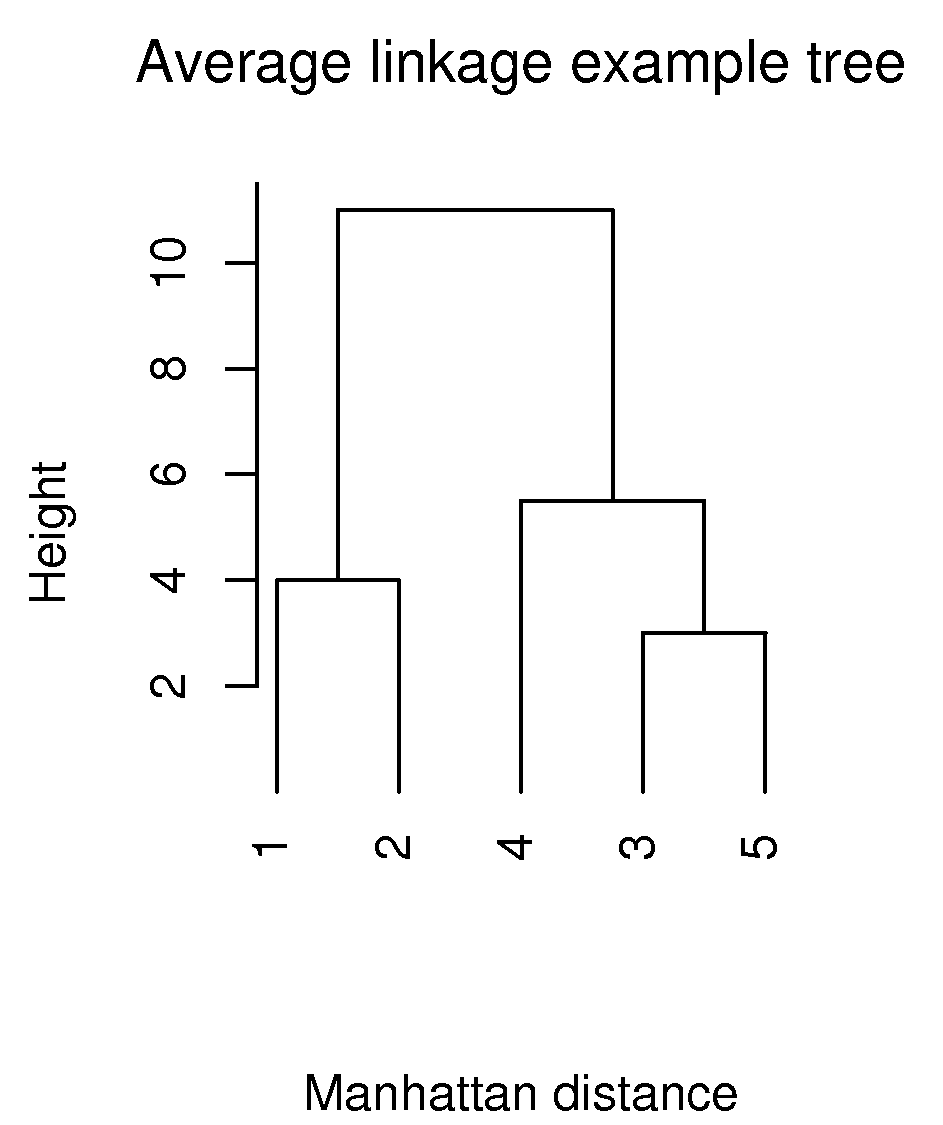
\includegraphics[scale=0.3]{Appendix/appendixtree.png}
\caption{Clustering  tree  for   5  bi-dimensional  vectors  using  the
  Manhattan  distance definition  and the  average  linkage clustering
  method.}
\label{fig:tree}
\end{figure}

\section{Clustering Validation Techniques}
\label{sec:validation}
The  main objective  of  automated  clustering methods  is  to find  a
reduced number  of groups which share common  characteristics within a
large dataset. The main problem  with the practical approaches used to
solve this task is that clustering  methods do not offer an 'a priori'
answer to  the optimal number  of groups that  a large dataset  can be
split into. In our simple example, shown in Figure \ref{fig:tree}, our
data split into two main  groups.  Since the assesment dependends upon
the distances and clustering methods used in particular cases, then an
emergent  necessity is  to be  able to  determine the  validity  of an
optimal number of clusters solution.  Clustering validation techniques
are thus crucial in the analysis of the gigantic amounts of data which
are  being  produced  in  the  the  post-genomic  boom  of  biological
information \cite{handl2005},  such as the structural  data dealt with
in this thesis.

We have used the  package clValid \cite{brock2008}, which implements a
variety  of clustering  validation algorithms,  using  the programming
language  \textbf{R}  \cite{rcite}.   The  clValid  package  comprises
measures which reflect  the compactness, connectedness, and separation
of cluster partitions. The concept  of compactness of a cluster refers
to the extent of  intra-cluster variation, the conectedness concept is
a more local  concept and means that neighboring  data elements should
belong to the same cluster,  and the separation concept quantifies the
degree of  separation between individual clusters.  An illustration of
these concepts is presented in Figure \ref{fig:concomsep}.

\begin{figure}
\centering
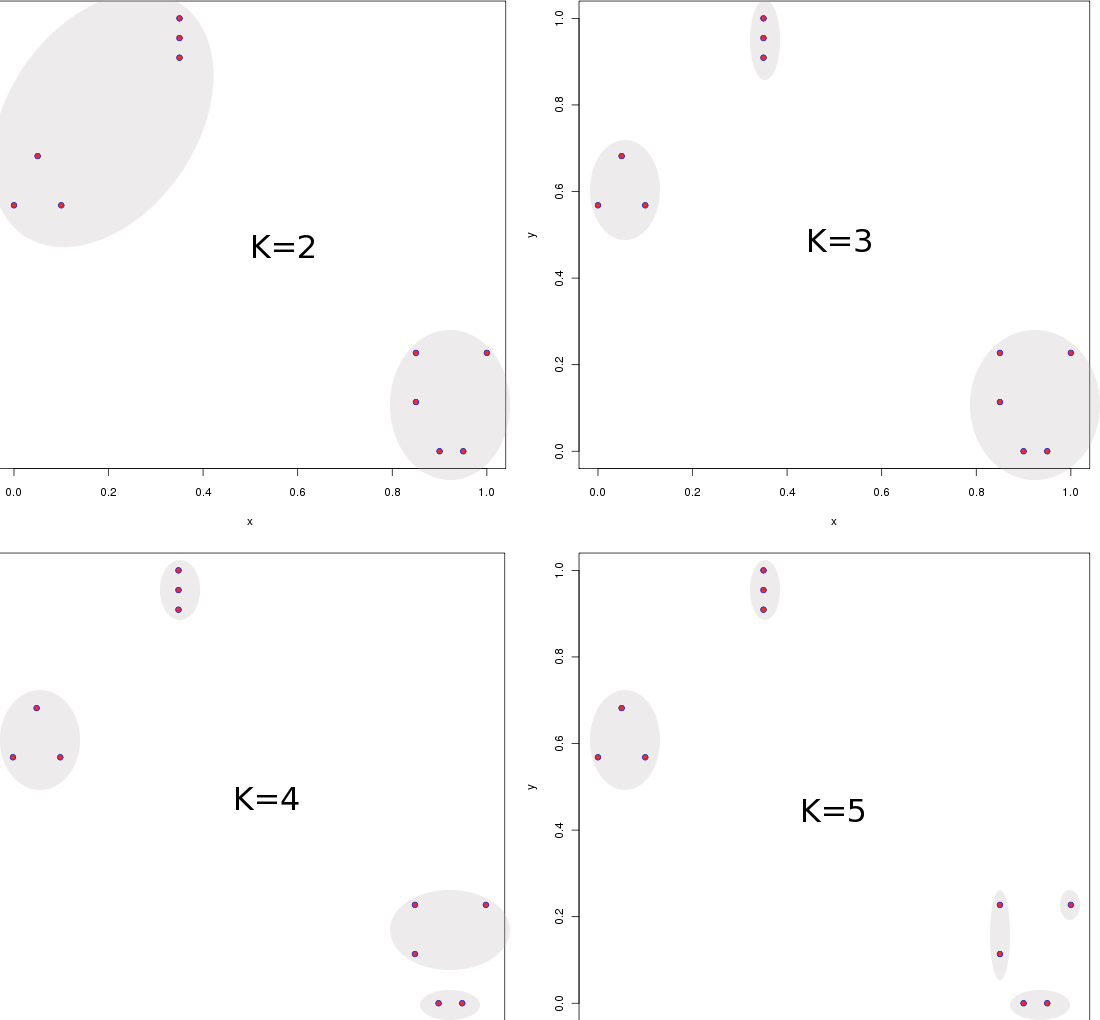
\includegraphics[scale=0.36]{Appendix/consilcom.png}
\caption{Illustration   of   the   compactness,   connectedness,   and
  separation  of  a bi-dimensional  dataset.  Images  a-d present  the
  solutions  for hierarchical  clustering of  the  euclidean distances
  between  the datapoints considering  $k=[2-5]$ clusters.   The $k=3$
  case, i.e.,  three clusters stands  out from the other  solutions in
  being composed of  more compact and separated groups.   This fact is
  quantified in clValid by the  \textit{asw} index and the Dunn index.
  The $k=2$  solution in (a),  by contrast, is clearly  more connected
  than all  other solutions.  One can  also see that  as the  data are
  grouped into  more clusters, the connectivity  will be progressively
  lost simply due to the splitting of the data.}
\label{fig:concomsep}
\end{figure}  

\subsection{Internal Measures}
There are two main types of measures in the clValid package, these are
called internal measures, and stability measures. In general, internal
measures are those that  use, exclusively, the dataset, the clustering
partitions,  and intrinsic  information in  the data  to  quantify the
quality of a  clustering result. In clValid three  indices are used to
account for compactness, conectedness and separation. The connectivity
index measures  cluster connectedness, while the  silhouette width and
Dunn  index provide combined  measures of  the cluster  separation and
compactness.

\subsubsection{Connectivity Index}
The connectivity index is defined as:
\begin{gather}
Conn(\mathcal{C}) = \sum_{i=1}^{N}\sum_{j=1}^{L} x_{i,nn_{i(j)}}
\end{gather}
Where   $nn_{i(j)}$   stands  for   the   $j^{th}$  nearest   neighbor
(\textit{nn}) to  the $i^{th}$ observation.  If $i$,  and its neareast
neighbor   $nn_{i(j)}$   are   in   the   same   cluster,   the   term
$x_{i,nn_{i(j)}}$ is zero. If they  do not belong to the same cluster,
then  the  term is  assigned  a value  of  $1/j$.   The parameter  $L$
resembles a radius,  in the sense that it  determines how many nearest
neighbors are taken into account per connectivity weight.
\begin{gather}
x_{i,nn_{i(j)}} =
    \begin{cases}
      0           &  \text{if } i \text{ and } nn_{i(j)} \in C_{k} \\
      \frac{1}{j} &  \text{otherwise.}
    \end{cases}
\end{gather}  
The  connectivity is  defined  for a  particular clustering  partition
$\mathcal{C} =  {C_{1},..., C_{K}}$, that is, for  a particular number
of clusters $k$ where the total number of observations is $N$. 
The connectivity index can give values between zero and infinity,
and smaller values mean better connectivity.

\subsubsection{Average Silhouette Width}
The  average  silhoutte  width  (\textit{asw})  is  the  mean  of  the
silhouette values $S(i)$ for $n$ observations,
\begin{gather}
\textit{asw} = \frac{1}{n} \sum_{i=1}^{n} S(i) \text{,}
\end{gather}  
Where the silhouette value is defined as:
\begin{gather}
\label{eq:silval}  
S(i) = \frac{b_{i}-a_{i}}{\max(a_{i},b_{i})} \text{.}
\end{gather}
Here  $a_{i}$ is  the average  dissimilarity of  observation  $i$ with
respect  to other  observations inside  the  cluster $i$  to which  it
belongs, and  $b_{i}$ is the average dissimilarity  of observation $i$
to the observations outside its own cluster, where $a_i$ and $b_i$ are
respectively defined as,
\begin{gather}
a_{i} = \frac{1}{n(C(i))} \sum_{j \in C(i)} d(i,j) \text{,}\\
b_{i}     =    \min_{C_{k}     \in     \mathcal{C}}    \sum_{j     \in
  C_{k}}\frac{d(i,j)}{n(C_{k})} \text{.}
\end{gather}  
The dissimilarity  $d(i,j)$ appearing in  the expression is  usually a
distance,  such  as  the  Euclidean or  Manhattan  distance,  although
formally  it  does  not  need   to  be  a  metric.   Notice  that  the
contributions to the  average silhouette width (\textit{asw}), defined
in  Equation  \ref{eq:silval}  can  only  have  values  in  the  range
$[-1:1]$.   According  to  Kaufman and  Rousseeuw  \cite{kaufman1990},
acceptable clusterings  usually have  an \textit{asw} value  above 0.5
and  those with  values below  0.2 should  be considered  as  not well
clustered. In this regard, it should  be noted that all the values for
validation   of   the    hierarchical   clustering   for   single-base
step-parameters  lie  above 0.5  in  the  lower  left plot  of  Figure
\ref{fig:internal}.

\subsubsection{Dunn Index}
The Dunn index is similar to  the \textit{asw} index in the sense that
it  also  quantifies  the  separation and  compactness  of  clustering
solutions.  It  is an  index  which  measures  the ratio  between  the
smallest inter-cluster distance and the largest intra-cluster distance
in a partitioning.  The index is defined by:
\begin{gather}
D(C) = \min_{C_{k} \in C} \left(  \frac{\min_{C_{l} \in C}
  d(C_{k},C_{l})}{\max_{C_{m} \in C} diam(C_{m})} \right)
\end{gather}
Where $\min_{C_{l \in C}} d(C_{k},C_{l})$ is the minimum inter-cluster
distance,  and  $\max_{C_{m}  \in   C}  diam(C_{m})$  is  the  maximum
intra-cluster distance.   The Dunn index can have  values between zero
and infinity, and a higher value means a better cluster separation and
compactness.

\subsection{Stability Measures}
Stability  measures are  a  special type  of  internal measure,  which
evaluate the consistency of a clustering result by comparing clustered
groups after sequential removal  of a column of data \cite{datta2003}.
In  the following  definitions  $N$  stands for  the  total number  of
datapoints  (rows of data)  and $M$  is the  total number  of columns,
dimensions  in the  data.  The  dimensions in  datapoints  usually are
taken as a  collection of samples or time  points.  These measures are
specially suited for  highly correlated data, as is  commonly the case
for high-throughput genomic data,  such as micro-arrays.  In the cases
shown here  an average is  taken over the  combined space of  the full
data and the reduced data sets.

\subsubsection{Average Proportion of Non-overlap (APN)}
The  average proportion  of  non-overlap  (APN) is  a  measure of  the
proportion of datapoints which are not placed in the same cluster when
a comparison is made between  full data clustering, and the clustering
performed  with one  column of  data, such  as one  type  of base-step
parameter, removed. Its value is defined as:
\begin{gather}
\text{APN}(\mathcal{C}) - \frac{1}{MN} \sum_{i=1}^{N}\sum_{l=1}^{M} \left( 1
- \frac{n(C^{i,j} \cap C^{i,0})}{n(C^{i,0})} \right) \text{,}
\end{gather}  
where $C^{i,0}$ is the cluster which contains datapoint $i$ in the
full dataset, and $C^{i,l}$ is the cluster which contains point $i$ in
the  reduced dimensionality  dataset, where  the column  $l$  has been
removed.  The  value of APN ranges between $[0-1]$  and is optimal
for values closer to zero \cite{datta2003, brock2008}.

\subsubsection{Average Distance (AD)}
The average distance (AD) measure computes the distance between datapoints in a
particular cluster of the full  dimensional dataset and that where one
column, or dimension has been removed,
\begin{gather}
AD(\mathcal{C})=\frac{1}{MN}       \sum_{i=1}^{N}\sum_{l=1}^{M}      -
\frac{1}{n(C^{i,0})n(C^{i,l})}  \left[  \sum_{i  \in  C^{i,0},  j  \in
    C^{i,l}} d(i,j) \right] \text{,}
\end{gather}
Here $d(i,j)$ is the distance between point $i$ in the full dimensional
dataset and point $j$ in the reduced dimension dataset.
The values of AD range between $[0-\infty]$ and are optimal when they
come closer to zero \cite{datta2003, brock2008}.

\subsubsection{Average Distance Between Means (ADM)}
The average  distance between means (ADM) score  measures the distance
between  the mean of  the datapoints  within a  cluster with  the full
number  of dimensions  and  the mean  of  the datapoints  of the  same
cluster when reduced by one dimension.
\begin{gather}
ADM(\mathcal{C})= \frac{1}{MN} \sum_{i=1}^{N} \sum_{l=1}^{M}
d(\bar{x}_{C^{i,l}}, \bar{x}_{C^{i,0}})
\end{gather}  
Here $\bar{x}_{C^{i,0}}$  is the mean  value of the datapoints  in the
cluster   which  contains  point   $i$  in   the  full   dataset,  and
$\bar{x}_{C^{i,l}}$ is the mean value of the datapoints in the cluster
containing point $i$ with column $l$ removed.  The values of ADM range
between $[0-\infty]$  and like the AD  and APN values  are optimal the
closer they are to zero \cite{datta2003, brock2008}.

%\newline
%Distance can be defined by Minkowski's metric:
%\begin{gather}
%d(X,Y)= \Big( \sum_{i=1}^N |x_i-y_i|^k \Big)^\frac{1}{k}
%\end{gather}
%In the particular case when $k=1$ we have the definition of the
%Manhattan or taxi-cab distance and when $k=2$ it's the familiar
%Euclidean distance.

%Finally, we can also define a maximum distance as the maximum
%difference between vectors variables.
%\begin{gather}
%d(X,Y) = max |x_{i}-y_{i}|
%\end{gather}

\bibliography{biblio}


